\documentclass[../main.tex]{subfiles}
\graphicspath{{\subfix{../img/}}}
\newacronym
  {pren1}                % id
  {PREN 1}                % display name
  {Produktentwicklung 1}  % full acronym name
  
\newacronym
  {pren2}                % id
  {PREN 2}                % display name
  {Produktentwicklung 2}  % full acronym name

\newacronym
  {yaml}
  {YAML}
  {YAML Ain't Markup Language}

\newacronym
  {tof-sensor}
  {ToF-Sensor}
  {Time-of-Flight Sensor}

\newglossaryentry{h-brücke}{
    name={H-Brücke},
    description={
         Eine H-Brücke ist eine Schaltung, die es ermöglicht, einen Elektromotor in beide Richtungen zu betreiben, indem sie den Stromfluss durch den Motor umkehrt. Sie besteht aus vier Schaltern (meistens Transistoren oder MOSFETs), die in einer "H"-Form angeordnet sind. Die Schalter werden so gesteuert, dass der Motor entweder vorwärts, rückwärts oder gestoppt wird.
    }
}


\newglossaryentry{pwm}{
    name={PWM},
    description={
        PWM (Pulsweitenmodulation) ist eine Technik zur Steuerung der Leistung von elektrischen Geräten, wie Motoren oder LEDs, durch das schnelle Ein- und Ausschalten eines Signals. Dabei wird die Dauer, in der das Signal "ein" ist (die Pulsbreite), im Vergleich zur Gesamtdauer eines Zyklus (der Periode) variiert.
    }
}


\newglossaryentry{ir-fototransistor}{
    name={IR-Fototransistor},
    description={
        Ein Fototransistor ist ein Halbleiterbauteil, das Licht in elektrischen Strom umwandelt. Wenn Licht auf den Transistor trifft, verändert sich seine elektrische Leitfähigkeit, was zu einer Stromänderung führt. Ein Infrarot(IR)-Fototransistor reagiert speziell auf Infrarotlicht. 
    }
}


\newglossaryentry{i2c}{
    name={I\textsuperscript{2}C},
    description={
        Eine serielle Kommunikationsschnittstelle, die den Datenaustausch zwischen verschiedenen Komponenten wie Mikrocontrollern, Sensoren und Aktoren über nur zwei Leitungen ermöglicht: \textit{Serial Data Line} für die Datenübertragung und \textit{Serial Clock Line} für die Synchronisation. 
        Die I\textsuperscript{2}C-Schnittstelle unterstützt mehrere Geräte in einem Netzwerk und verwendet Adressen, um einzelne Komponenten anzusprechen.
    }
}


\newglossaryentry{uart}{
    name={UART},
    description={
        Abkürzung für \textit{Universal Asynchronous Receiver Transmitter}. 
        Eine Hardware-Komponente oder ein Kommunikationsprotokoll, das zur seriellen, asynchronen Datenübertragung verwendet wird. 
        UART ermöglicht die Kommunikation zwischen zwei Geräten, indem Daten über eine Sendeleitung (\textit{TX}) und eine Empfangsleitung (\textit{RX}) übertragen werden. Es erfordert keine gemeinsame Taktleitung und verwendet stattdessen Start- und Stoppbits zur Synchronisation. 
    }
}


\newglossaryentry{PLA}{
    name={PLA},
    description={
    Polymilchsäure   (PLA) ist ein biologisch   abbaubarer, thermoplastischer Kunststoff, der aus erneuerbaren Ressourcen wie Maisstärke oder Zuckerrohr hergestellt wird.
    }}

\begin{document}

\newpage
\section{Reflexion zur Nachhaltigkeit}

\begin{figure}[H] % 'h' steht für here, was bedeutet, dass das Bild möglichst an dieser Stelle eingefügt wird
    \centering
        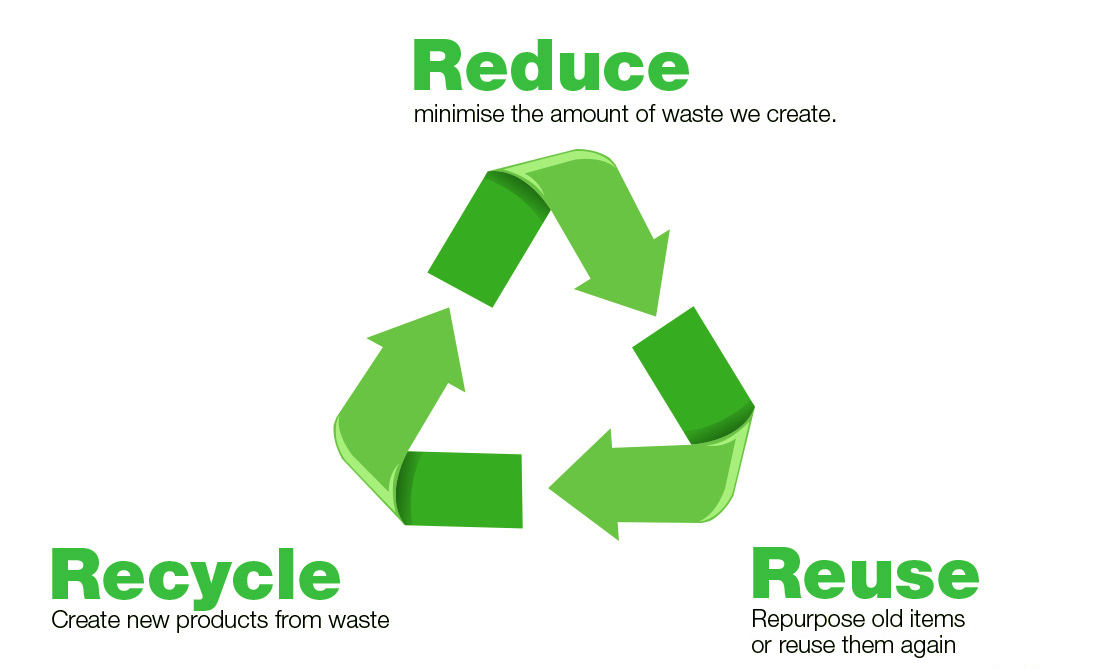
\includegraphics[width=0.7\linewidth]{img/nachhaltigkeit/3R-reduce-reuse-recycle.jpg}
        \caption[Nachhaltigkeits-Prinzip: Reduce, Reuse, Recycle]{Nachhaltigkeits-Prinzip: Reduce, Reuse, Recycle \footnotemark}
        
        \label{fig:3R}
    \end{figure} 

    \footnotetext{Quelle: \url{https://innovation-yachts.com/3r-reduce-reuse-recycle/}}

Nachhaltigkeit spielt eine zunehmende, zentrale Rolle in der Produktentwicklung, insbesondere im Bereich Maschinenbau und Automation. In diesem Projekt werden die Prinzipien der Nachhaltigkeit bewusst berücksichtigt, um einen positiven Beitrag zur Umwelt zu leisten und die Ressourcennutzung zu optimieren.

\subsection{Reduce – Ressourcen minimieren}

Ein Schwerpunkt dieser Arbeit liegt darin, den Materialverbrauch und den Energiebedarf zu reduzieren. Schon in der Konzeptphase werden Designs entwickelt, die mit wenigen Komponenten auskommen. Ziel ist es, den Materialeinsatz so gering wie möglich zu halten. Dabei wird ein grosses Augenmerk auf die Einsparung von Elektrokomponenten gelegt. Die Entscheidung fällt auf ein Konzept, welches mit lediglich zwei Fahrantrieben und nur einem Antrieb für die gesamte Hindernisbewältigung auskommt. Durch ein rein mechanisches System werden Sensoren und weitere Antriebe eingespart. Auch beim Prototyping wird darauf geachtet, nur Teile herzustellen, welche effektiv für Tests vonnöten sind. Es wird darauf geachtet, die benötigten Komponenten für das gesamte Projekt bei Schweizer Anbietern zu bestellen, siehe Tabelle \ref{tab:ausgaben_pren1}.

\subsection{Reuse – Wiederverwendbarkeit fördern}

Ein weiteres Ziel war es, die Wiederverwendbarkeit der Komponenten zu erhöhen. Modulare Bauweisen und standardisierte Schnittstellen wurden implementiert, um eine einfache Demontage und Wiederverwendung einzelner Bauteile zu ermöglichen. Vor der Bestellung von Bauteilen wurde jeweils geprüft, ob eine Übernahme von Komponenten aus früheren Pren-Durchführungen möglich war. Bei der Konzeption von Testaufbauten wurde insbesondere darauf geachtet, bereits vorhandene Komponenten zu nutzen. Im Rahmen der Testung der Motoren wurde ein Chassis aus einer alten Holzplatte gefertigt, anstatt ein neues Chassis zu drucken.

\subsection{Recycle – Wiederverwertung ermöglichen}

Bei der Materialauswahl wird auf die Verwendung recyclingfähiger Materialien geachtet, um eine umweltgerechte Entsorgung sicherzustellen. Die Vermeidung von Verbundwerkstoffen und der Einsatz sortenreiner Materialien erleichtern die Rückgewinnung und Wiederverwertung am Ende der Produktlebensdauer. Gleichzeitig wird bei der Entwicklung darauf geachtet, möglichst wenig Produktionsabfälle zu generieren, und diese gezielt dem Recycling zuzuführen. So wird das Chassis aus Aluminium gefertigt, was zu 100 \% recyclebar ist. Für die Herstellung von 3D-Druckteilen wird \gls{PLA} verwendet. Dieses Material basiert auf Maisstärke und hat eine geringere Umweltbelastung als erdölbasierte Kunststoffe. Zudem kann PLA unter kontrollierten Bedingungen biologisch abgebaut werden, was es zu einer umweltfreundlichen Alternative macht.

\subsection{Ergebnis Nachhaltigkeit}

Durch die Integration der Prinzipien \textbf{Reduce, Reuse, Recycle} (Abb.\ref{fig:3R}) ist es möglich, die Nachhaltigkeit eines Produktes zu verbessern. Die Umsetzung dieser Strategien hat nicht nur ökologische Vorteile, sondern trägt auch zur Kostenreduktion bei. Dieses Projekt zeigt, dass nachhaltige Entwicklung und technologische Innovation Hand in Hand gehen können und einen langfristigen Mehrwert schaffen.

Diese Reflexion verdeutlicht, dass Nachhaltigkeit nicht nur ein Ziel, sondern ein integraler Bestandteil des Entwicklungsprozesses ist, der auch in PREN2 konsequent weiterverfolgt wird.


\end{document}